On considère les fonctions $f_{k}$ définies sur $\R$ par 
\[f_{k}(x) = x + k \e^{-x},\]
 où $k$ est un réel strictement positif.

	\begin{enumerate}
		\item On s'intéresse dans cette question au cas $k = 0,5$, donc à la fonction $f_{0,5}$ définie sur $\R$ par :
\[f_{0,5}(x) = x + 0,5 \e^{-x}.\]

\smallskip
	\begin{enumerate}
		\item Montrer que la dérivée de $f_{0,5}$, notée $f'{ }_{0,5}$ vérifie $f'{ }_{0,5}(x) = 1-0,5 \e^{-x}$.

		\item Montrer que la fonction $f_{0,5}$ admet un minimum en $\ln (0,5)$.
	\end{enumerate}
\end{enumerate}

		Soit $k$ un réel strictement positif. On donne le tableau de variations de la fonction $f_{k}$.
		\medskip
		

					\hfill~\begin{tikzpicture}
				\tkzTabInit[lgt=3]{Valeurs de $x$/0.7,
					Variations de $f_k$/1.5}{$-\infty$,$\ln(k)$,$+\infty$}
				\tkzTabVar{+/$+ \infty$,-/$f_k(\ln k)$,+/$+\infty$}
			\end{tikzpicture}\hfill~

	\begin{enumerate}
		\setcounter{enumi}{1}
		\item Montrer que pour tout réel positif $k, f_{k}(\ln k) = \ln k + 1$.
	\end{enumerate}

On note $\mathcal{C}_{k}$ la courbe représentative de la fonction $f_{k}$ dans un plan muni d'un repère orthonormé.

On note $\mathrm{A}_{k}$ le point de la courbe $\mathcal{C}_{k}$ d'abscisse $\ln k$.

On a représenté ci-dessous quelques courbes $\mathcal{C}_{k}$ pour différentes valeurs de $k$.

	\begin{center}
			\begin{center}
				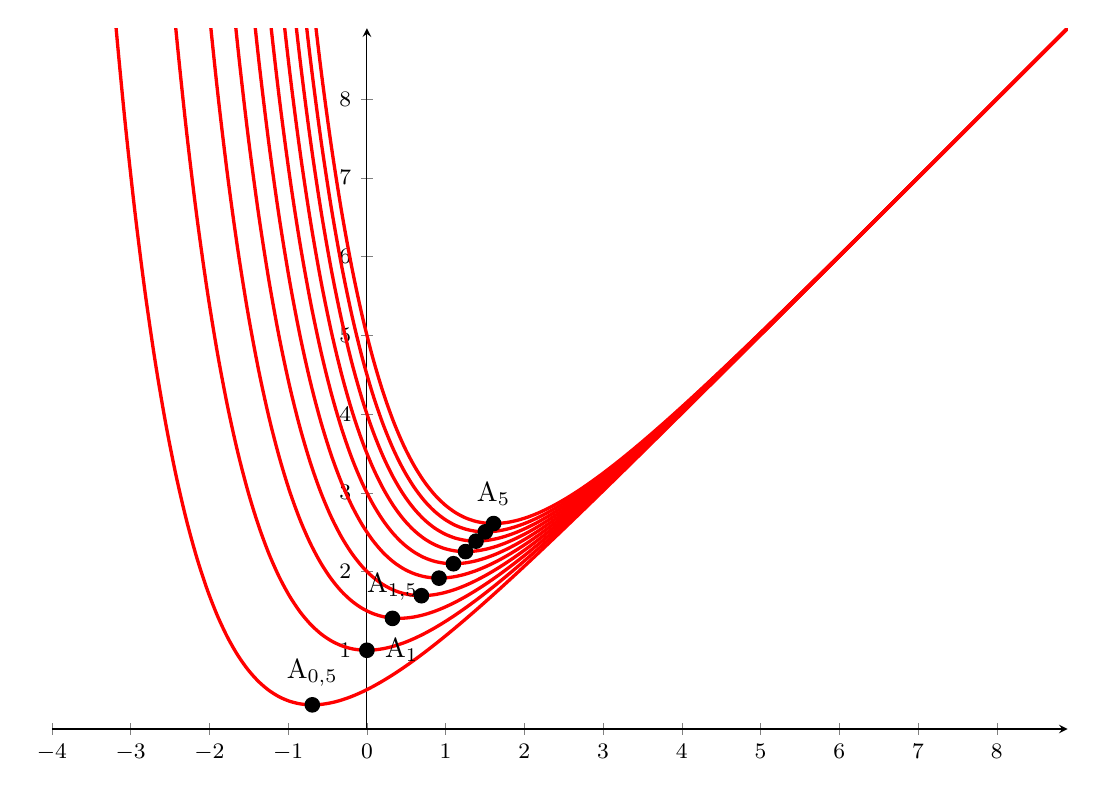
\begin{tikzpicture}
					\begin{axis}[x={10mm},y={10mm},    xmin=-4,  xmax=8.9,    ymin = 0,     ymax=8.9, xtick distance=1,    ytick distance = 1,
						tick label style={font=\footnotesize}, minor tick num = 0, grid=none,  axis y line=center,axis x line=bottom]
						\foreach \coef in{0.5,1,1.5,2,2.5,3,3.5,4,4.5,5}
						{\addplot [line width=1.2pt, color=red, smooth, samples=100, domain= -4:9 ]{x+\coef*exp(-x)};}
				\node[label={90:{$\mathrm{A}_{0,5}$}},circle,fill,inner sep=2pt] at (axis cs:-0.693,0.307) {};
				\node[label={0:{$\mathrm{A}_1$}},circle,fill,inner sep=2pt] at (axis cs:0,1) {};
				\node[label={90:{$\mathrm{A}_{1,5}$}},circle,fill,inner sep=2pt] at (axis cs:0.325,1.405) {};
				\node[circle,fill,inner sep=2pt] at (axis cs:0.693,1.693) {};
				\node[circle,fill,inner sep=2pt] at (axis cs:0.916,1.916) {};
				\node[circle,fill,inner sep=2pt] at (axis cs:1.099,2.099) {};
				\node[circle,fill,inner sep=2pt] at (axis cs:1.253,2.253) {};
				\node[circle,fill,inner sep=2pt] at (axis cs:1.386,2.386) {};
				\node[circle,fill,inner sep=2pt] at (axis cs:1.504,2.504) {};
				\node[label={90:{$\mathrm{A}_5$}},circle,fill,inner sep=2pt] at (axis cs:1.609,2.609) {};
			\end{axis}
				\end{tikzpicture}
			\end{center}
		\end{center}

\begin{enumerate}
		\setcounter{enumi}{2}
		\item Indiquer si l'affirmation suivante est vraie ou fausse. Justifier la réponse. Une réponse non justifiée ne rapporte aucun point.

		\begin{itemize}
		\item \textbf{Affirmation :} \og{}Pour tout réel $k$ strictement positif, les points $A_{0,5}, A_{1}$ et $A_{k}$ sont alignés. \fg{}
		\end{itemize}
\end{enumerate}
